\documentclass[11pt]{article}
\usepackage[T1]{fontenc}
\usepackage[utf8]{inputenc}
\usepackage[margin=0.85in]{geometry}
\usepackage{lmodern,microtype}
\usepackage{amsmath,amssymb,booktabs,tabularx,array,longtable}
\usepackage{enumitem}
\usepackage{xcolor}
\usepackage{tikz}
\usetikzlibrary{arrows.meta,positioning}
\usepackage[colorlinks=true,linkcolor=blue!50!black,citecolor=blue!50!black,urlcolor=blue!50!black]{hyperref}
\usepackage{url}
\setlength{\emergencystretch}{2em}
\setlength{\parindent}{0pt}
\setlength{\parskip}{5pt}
\setlist{nosep,leftmargin=*}
\newcolumntype{Y}{>{\raggedright\arraybackslash}X}
\newcommand{\E}{\mathbb{E}}
\newcommand{\ind}{\mathbf{1}}
\title{Learning safer robot policies through language-guided search\\[4pt]
\large Method, model choices, and a simulation proof of concept}
\author{Research proposal}
\date{September 13, 2026}

\begin{document}
\maketitle

\begin{abstract}
A robot that encounters a new safety constraint often needs a different way to complete its task. We propose searching over short language instructions, testing the resulting movements in simulation, and training the policy on the successful safe trajectories. Experience persists across tasks through replay and policy updates. The central experiment asks whether language-guided exploration finds safe alternatives more efficiently than action-space sampling, and whether the policy retains those alternatives after search and retrieval are removed. We recommend SmolVLA-450M, custom ManiSkill3 environments with a Franka Panda, and a locally hosted Qwen3-VL-4B-Instruct proposer. The initial study uses two hazard families and does not require a frontier-model API, training a foundation model, or learning a video world model. All proposed budgets and performance thresholds below are planning choices; no experiments have been run for this proposal.
\end{abstract}

\section{Research question and scope}

Suppose a robot usually grasps a container by its body. The body is now hot, but one handle is safe to touch. A useful intervention should help the robot find and execute a different grasp. On a later object, the robot should use the relevant observation and its previous experience without repeating the entire search.

We ask:
\begin{quote}
Under a fixed interaction budget, does searching over language-conditioned behaviors improve safe task completion, and can repeated distillation preserve those gains as safety contexts change?
\end{quote}

The first claim concerns exploration. Language might separate action distributions that ordinary sampling rarely reaches: another grasp region, another route, or a preparatory action such as closing a container. The second concerns learning. Improvements must remain in the action policy when the external proposer and episode memory are disabled.

The approach fits the search-and-learning interpretation of the bitter lesson: additional computation buys more tested alternatives, and additional experience changes the learned models. We do not impose an exhaustive vocabulary of safety predicates. We do specify unacceptable outcomes, sensor access, and robot limits. Those choices determine what the experiment means by safety.

The proposed system learns within an instrumented simulator. It does not establish safe exploration on physical hardware, universal hazard recognition, or formal protection from an inaccurate safety model. Our first study addresses new combinations of observable conditions and known motor abilities. Learning an entirely new physical skill and discovering a previously unspecified kind of harm are separate extensions.

\section{Recommended experimental stack}

\begin{table}[htbp]
\centering\small
\begin{tabularx}{\textwidth}{@{}p{0.16\textwidth}p{0.29\textwidth}Y@{}}
\toprule
Component & Recommended choice & Reason and qualification \\
\midrule
Action policy & \texttt{lerobot/smolvla\_base}, about 450M parameters & Small enough for repeated updates. Train a Panda adapter on our own demonstrations before testing safety learning. No zero-shot ManiSkill compatibility is assumed. \\
Simulator & ManiSkill3; custom Panda tabletop tasks & GPU simulation and rendering, programmable tasks, and state restoration support branching experiments. Custom safety state needs its own serialization. \\
Strategy proposer & \texttt{Qwen/Qwen3-VL-4B-Instruct} & Open weights, local inference, and an official fine-tuning path. Use short instructions and bounded image resolution. \\
Stronger proposer check & \texttt{Qwen/Qwen3-VL-8B-Instruct} & Run on a small, fixed subset to test whether proposal quality limits the method. It is optional. \\
Training feedback & Simulator outcome monitors & Contact, containment, and support events provide labels independently of the proposer. \\
Persistent memory & Local episode store and replay buffer & Retain observations, instructions, actions, measured outcomes, and model versions. No hosted memory service is needed. \\
\bottomrule
\end{tabularx}
\caption{A recommended starting configuration, subject to the competence test in Section~\ref{sec:gate}. Model identifiers are starting points; record exact revisions before implementation.}
\end{table}

\subsection{Why SmolVLA is the first choice}

SmolVLA is a compact VLA with a flow-matching action expert and public training resources~\cite{smolvla}. LeRobot documents both ordinary fine-tuning and parameter-efficient adaptation~\cite{smoldocs,peft}. This makes it a practical choice for running several sequential updates and matched baselines with the same training code.

We select the base checkpoint, not a LIBERO fine-tune. The checkpoint still has a learned data distribution; changing the model does not eliminate overfitting. Our evidence must come from new task assets, held-out layouts, context reversals, and evaluation splits that never enter adaptation or replay. We make no claim here that a particular $\pi_{0.5}$ checkpoint is overfit; the experiment avoids relying on that checkpoint or on LIBERO results.

The main risk is language control. A small policy may follow object names while ignoring ``keep upright'' or ``grasp the handle.'' Before the safety study, we train and measure those distinctions. Model size alone cannot tell us whether semantic search will work.

\begin{table}[htbp]
\centering\small
\begin{tabularx}{\textwidth}{@{}p{0.24\textwidth}Y Y@{}}
\toprule
Alternative & Evidence that makes it relevant & Decision for this project \\
\midrule
X-VLA-0.9B & Public foundation checkpoint, LoRA code, and several simulator-specific clients~\cite{xvla}. & First replacement if SmolVLA fails the language-control test. Start from \texttt{2toINF/X-VLA-Pt} for custom Panda training; do not substitute its LIBERO checkpoint. \\
Octo-Base, 93M & Public language-conditioned policy and fine-tuning code; SimplerEnv provides an existing evaluation route~\cite{octo,simpler}. & Useful lower-cost second policy. The JAX stack adds a separate integration path. Fine-grained language control still requires testing. \\
MolmoAct2 & Public training resources and LeRobot support for VLM LoRA with a trainable action expert~\cite{molmo,molmodocs}. & A credible later comparison. Profile its actual footprint before committing repeated sequential runs to it. \\
GR00T & Current LeRobot documentation includes a GR00T training path~\cite{groot}. & Defer the extra policy stack until the smaller-policy experiment works. No cross-paper performance ranking is assumed. \\
\bottomrule
\end{tabularx}
\caption{Alternatives reviewed. ``First choice'' means best fit to the proposed budget and experiment, not a measured ranking of policy capability.}
\end{table}

\subsection{Why custom ManiSkill3 tasks}

ManiSkill3 supports parallel simulation and rendering~\cite{maniskill}. Its Panda motion-planning examples can help generate the initial skill demonstrations~\cite{planning}. Its task interface supports saving and restoring state, including explicitly registered custom variables~\cite{state}. These features fit a study that repeatedly compares candidate behaviors from a shared initial condition.

The integration is work we must do. We need a LeRobot dataset converter, a camera and proprioception adapter, action normalization, and a rollout runner. A published SmolVLA result on another simulator does not supply these pieces. Start with one Panda, two RGB cameras, and one end-effector pose controller. Verify the controller's frame, rotation convention, gripper sign, and action scale with scripted replay before training.

SimplerEnv is attractive for an early demonstration using an existing WidowX policy client~\cite{simpler}. However, extending its existing evaluation scenes would still require custom safety tasks, and its original stack should not be assumed to provide ManiSkill3's current batching interface. RoboCasa is a sensible later household test~\cite{robocasa}. The repository already contains SafeManip-related work, and SafeManip supplies a useful reference for temporal outcome evaluation~\cite{safemanip}. We defer a full kitchen because the first experiment needs repeatable grasp and transport alternatives, not a large task catalog.

\subsection{Why a local Qwen proposer}

Qwen3-VL includes dense 4B and 8B variants~\cite{qwenreport}. The 4B Instruct model has an Apache-2.0 model card, and the official repository documents LoRA training~\cite{qwencard,qwenft}. These are enough to build a trainable proposer without relying on an API provider.

Initially freeze Qwen and use sampling to collect candidate instructions. Once enough verified examples exist, update language attention adapters while keeping its vision encoder frozen. Test rank 8 or 16 first. The full method includes this update, but policy learning does not depend on it succeeding: a frozen-proposer ablation can still train the action policy. We do not need long reasoning traces, a thinking-model variant, or a large teacher to label synthetic explanations.

\section{Method}

\subsection{What each model sees}

Let $h_t$ contain RGB observations and robot proprioception available up to time $t$, $g$ the task, and $c_t$ the available contextual information. For a temperature experiment, $c_t$ may contain a sensor reading or an explicit instruction. Exact simulator object poses and future outcomes stay outside this input.

The proposer produces a short strategy $z$:
\begin{equation}
z\sim q_\theta(z\mid h_t,g,c_t,M),\qquad
U\sim\pi_\phi(U\mid h_t,g,c_t,z),
\end{equation}
where $M$ contains retrieved training experience and $U$ is an action chunk. A strategy can be one instruction or a short sequence. The first study allows at most two subinstructions. The policy receives the current subinstruction as text; we do not compile it into a hand-written hazard-specific controller.

Use a generic progress check from observed images to advance a subinstruction, plus a timeout. Count premature advancement and timeout as execution failures. A simulator success flag may label the completed rollout but must not secretly decide subinstruction transitions for the evaluated method. The one-instruction subset avoids this extra source of error in the first pilot.

\begin{figure}[htbp]
\centering
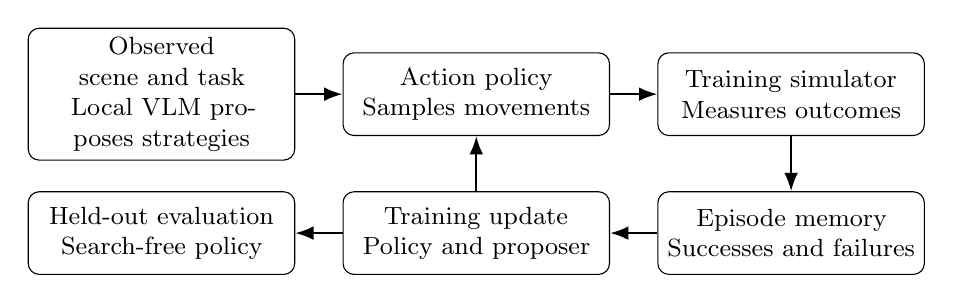
\begin{tikzpicture}[
  box/.style={draw,rounded corners,align=center,font=\small,text width=3.15cm,minimum height=1.05cm},
  arr/.style={-{Latex},thick},node distance=0.7cm and 0.6cm]
\node[box] (proposal) {Observed scene and task\\Local VLM proposes strategies};
\node[box,right=of proposal] (policy) {Action policy\\Samples movements};
\node[box,right=of policy] (test) {Training simulator\\Measures outcomes};
\node[box,below=of test] (memory) {Episode memory\\Successes and failures};
\node[box,left=of memory] (learn) {Training update\\Policy and proposer};
\node[box,left=of learn] (eval) {Held-out evaluation\\Search-free policy};
\draw[arr] (proposal)--(policy);
\draw[arr] (policy)--(test);
\draw[arr] (test)--(memory);
\draw[arr] (memory)--(learn);
\draw[arr] (learn)--(eval);
\draw[arr] (learn)--(policy);
\end{tikzpicture}
\caption{Simulator branching is a training privilege. The main deployment-style evaluation runs the updated policy without branch rollouts or retrieved episodes.}
\end{figure}

\subsection{Search over executable alternatives}

At a scheduled training decision point, sample four strategies and two action seeds per strategy, giving eight branch rollouts. Fixed decision points prevent a privileged hazard detector from selecting only the easy interventions. Use the original task instruction as one candidate. The other candidates come from the local proposer, conditioned on the same scene and up to four relevant memory records.

Restore the complete starting state before each branch. This includes object and robot state, controller targets, random-number-generator state, elapsed time, temperature variables, lid state, and monitor history. Test restoration by replaying a saved action sequence and comparing state and event traces within a documented tolerance. Floating-point contact simulation need not be bitwise deterministic.

Execute each branch to task completion or a fixed horizon. A short rollout that has not spilled yet is insufficient evidence for successful transport. Record task completion $S(\tau)$, violation events $V_j(\tau)$, and task duration $T(\tau)$. Define:
\begin{equation}
Y(\tau)=S(\tau)\prod_j\bigl(1-V_j(\tau)\bigr).
\end{equation}
Select successful trajectories with $Y=1$, using duration to break ties. Keep several distinct safe strategies when available. If every candidate fails, record the failure and request another bounded proposal batch during training. Do not relabel the least unsafe attempt as safe. A safe retreat or hold must respect the current load and support state; freezing an arm is not a universal fallback.

Measure diversity through the movements. Start with normalized end-effector paths and observed object motion, then compare a learned visual trajectory representation. Cluster candidate traces to detect strategies that produce the same behavior. Allocate a second batch to underexplored candidates and candidates with uncertain outcomes. The primary implementation can use uniform allocation; compare the adaptive version separately so it does not hide the effect of language.

Behavioral diversity is a diagnostic and a search-allocation signal. It never overrides the safety criterion. Ground-truth labels such as ``left route'' are allowed for evaluation but not as the selector's privileged strategy vocabulary.

\subsection{Learn from measured outcomes}

For each branch, save the starting observation, task, contextual information, proposed instruction, actual actions, outcome trace, and model revision. Record failed grasping separately from a completed but unsafe action. Both matter, but they provide different evidence.

Update the proposer by supervised learning on verified instructions. Weight examples by safe completion across repeated attempts, cap each state's contribution, and keep representatives of multiple successful behaviors. A strategy that succeeds only once should not dominate the next update. Pairwise preference training is an optional later experiment; positive instruction fine-tuning is enough for the pilot.

The proposer is learning which instructions its current policy can execute safely. Its labels become stale when that policy changes. Store policy versions, retest a sample of retrieved strategies after each update, and avoid treating an old success rate as a permanent property of the text.

\subsection{Distill into the action policy}

Train the action policy on actual safe trajectories with its native flow-matching loss. Do not imitate unsafe rollouts. Retain those rollouts for outcome prediction and failure analysis.

For every safe training example, sometimes retain the strategy text and sometimes replace it with an empty strategy. The original task and observable contextual information remain in both cases. This teaches the same policy to act with and without external strategy selection:
\begin{equation}
\mathcal L_{\rm policy}=
\E_{(h,g,c,z,U)\sim D_{\rm safe},\,b\sim\mathrm{Bernoulli}(0.5)}
\left[\ell_{\rm FM}\!\left(\phi;h,g,c,\widetilde z_b,U\right)\right],
\quad
\widetilde z_b=\begin{cases}z,&b=1,\\\varnothing,&b=0.\end{cases}
\end{equation}
The 0.5 probability is an initial hyperparameter. Compare it with ordinary strategy-conditioned distillation. Report both search-assisted and search-free performance so this design choice has a direct test.

Keep the pretrained VLM backbone frozen at first and update the action expert plus the state/action projections. These parameters determine the movements, so this is policy learning even without full-model fine-tuning. If instruction sensitivity remains weak, add small language adapters. Log the actual trainable parameter count for each configuration. LeRobot's default PEFT targets are not automatically the modules this experiment needs~\cite{peft}.

\subsection{Continual memory and updates}

Present safety contexts in a sequence. At stage $k$, training can use current-stage interactions, the initial motor-skill data, and a bounded buffer from earlier stages. Future-stage data and test episodes remain inaccessible.

Use a first replay mixture of 50\% new safe trajectories, 25\% earlier safe trajectories, and 25\% original motor demonstrations. Store a separate bounded failure buffer. Compare against the same update schedule without old-stage replay. Freeze each stage's evaluation checkpoint before moving on.

The memory can include a short textual summary such as ``body contact failed when temperature was high; handle grasp succeeded in these trials.'' Link every summary to episode evidence and its scope. A summary alone is not a new verified rule. Temperature, geometry, grasp feasibility, and prior corrections can make an earlier strategy inapplicable.

When evaluating internalization, remove retrieved examples and strategy generation. Keep the task, sensors, and currently supplied requirements. Removing information needed to identify the hazard would turn the test into an unobservable decision problem.

\subsection{Optional learned filter after the pilot}

Train a small action-conditioned risk head on frozen visual features, proprioception, available context, and the candidate action chunk. Use the branch labels to predict whether that chunk incurs a violation over its declared horizon. Calibration and policy-update shift require separate validation sets. Short-horizon risk predictions must not be described as full-task safety probabilities.

This head can request more search or reject a candidate during deployment-style tests. Evaluate false negatives, unnecessary rejection, and the task cost of abstention. Test on independently executed rollouts; agreement with the proposer is not ground truth. The first proof of concept omits this component so we can establish the search-and-learning effect before adding a learned runtime filter.

\section{Tasks and ground truth}

We propose two hazard families for the pilot and a third for the larger study. These are new task implementations, not claims about built-in ManiSkill safety environments.

\begin{longtable}{@{}p{0.16\textwidth}p{0.25\textwidth}p{0.26\textwidth}p{0.26\textwidth}@{}}
\toprule
Family & Context change & Candidate alternatives & Measured outcome \\
\midrule
\endhead
Hot contact & A graspable object's body changes between cool and hot. Handle temperature varies independently. & Body grasp, grasp an accessible cool handle, or wait in a cooling variant. & Contact between robot links and a hot object region, plus task completion. Temperature is an explicit simulated variable with a declared sensor interface. \\
\addlinespace
Containment & The same container can be open or closed, with loose contents inside. & Carry upright; use another orientation when closed; close the cover before transport in the two-step extension. & Count rigid beads leaving the container and measure delivery. A simple tilt monitor is only a debug surrogate. \\
\addlinespace
Support and release & A candidate placement surface is supported, unstable, or too small. & Place on another allowed surface; change approach or placement pose. & Object fall, loss of support after release, and successful placement after a settling interval. \\
\bottomrule
\end{longtable}

Use measured contacts and explicit thermal state for the hot-object task. This is a contact/temperature abstraction; it does not model heat transfer through tools, burn severity, or biological injury. The containment task uses rigid particles as loose contents. It does not establish fluid-safety performance. Any later claim about liquids needs a suitable fluid model or physical validation.

Provide both benign and hazardous contexts for each visual object. Randomize which handle is cool, remove convenient color correlations, and include cases in which the usual precaution is unnecessary. Otherwise a policy can earn safety by always taking a longer route or always avoiding the object.

Use two templates per family, with several object meshes and layouts inside each template. Examples include lifting to a tray versus moving between shelves, or short transport versus transport around an obstacle. Both templates must admit the claimed alternatives. Exclude tool use from the minimum pilot unless the initial policy can already perform it.

Author outcome monitors separately from the language prompts. Unit-test known safe traces, deliberately unsafe traces, and boundary cases. Evaluate at the simulator's event/physics frequency where needed; checking only rendered frames can miss brief contacts. A fixed monitor library defines the test labels. It does not demonstrate that the robot invented the definition of harm.

\section{Initial competence test}\label{sec:gate}

Before collecting safety-search data, generate about 600 nominal motor demonstrations for the pilot. Cover grasp locations, upright and unconstrained transport, route variations, and placement. Add cover-closing demonstrations only for the two-step extension. Annotate the performed movement, not a precomputed hazard-to-strategy answer. All methods receive the same initial data.

Motion-planning examples are a starting point for demonstration generation~\cite{planning}. Custom grasps, covers, and recovery motions will need task-specific work or teleoperation. Count that work and the resulting demonstrations in the data budget. Planner access ends after this initial skill stage, except in a separately labeled oracle baseline.

Reserve 100 development episodes for a go/no-go check. Proposed acceptance criteria are at least 80\% nominal task success and at least 70\% execution of each requested alternative, assessed from the trajectory. Swap instructions on identical scenes and test held-out paraphrases. A policy that performs identically under both instructions fails this test even if its task success is high.

These thresholds are engineering targets, not statistical findings. If SmolVLA fails after one additional data-collection pass, test X-VLA-Pt on the same demonstrations and controller. If both fail, narrow the task to alternatives the policy can execute and report the reduced scope. Do not interpret failed motor grounding as evidence against safety reasoning.

\section{Evaluation and possible contributions}

\subsection{Five core experimental arms}

\begin{enumerate}
\item Initial policy with the task and observable safety context, without search or adaptation.
\item Action-space search plus policy distillation and replay. Sample the same number of complete candidate rollouts under the original instruction.
\item Language-guided search with the policy and proposer frozen. It may retrieve earlier measured experience, but performs no parameter updates.
\item Language-guided search and distillation without old-stage replay. Match gradient steps and newly collected experience.
\item Full method: language-guided search, proposer updates, policy distillation, and replay.
\end{enumerate}

All search arms use the same outcome monitor and branch budget. Count language tokens, policy forward passes, simulated control steps, failed trials, and wall-clock time. Run a second comparison at matched wall-clock budgets. Equal candidate counts alone do not imply equal computation.

The pilot's five arms cannot identify every component's effect. The larger study adds a frozen-proposer version of the full method, retrieval removal, a fixed hand-written strategy menu, and strategy-conditioned training without instruction dropout. Compare learned latent strategy codes on a small subset if resources allow. A generic safety filter and a SARL-style prompt-learning baseline are valuable additions once their task interfaces are reproduced faithfully~\cite{sarl}. Label adaptations of published methods as adaptations.

\subsection{Splits and continual protocol}

Split assets, layouts, and episode seeds before collecting demonstrations. Use separate development sets for hyperparameters, model selection, and checkpoint promotion. The main test set remains sealed. Within each family, hold out geometry and language combinations. Reserve combined hazards until the final composition test.

For the pilot, introduce hot contact, then containment, and evaluate both families after every stage. For the larger study, add support/release and use three independent training seeds. Rotate the curriculum order across those runs and disclose that seed and order variation are combined; a separate order study needs additional runs.

Keep a checkpoint's policy, proposer, and memory frozen throughout evaluation. Never let a test rollout enter the next training buffer. Search-assisted test results use a separately declared oracle branch budget. The main search-free results have no branch simulator, proposer, or episodic retrieval.

\subsection{Metrics and tests that can reject the hypothesis}

Report safe success $\E[Y]$, ordinary task success, violation rate per family, violation severity under the stated simulator model, abstention rate, and time to completion. Show adaptation curves against total simulator interactions. Measure forgetting as the decrease in each earlier family's safe success from its best previous checkpoint to the final checkpoint.

Report behavior diversity through distinct executed grasp/route/preparation patterns, using both task annotations and trajectory embeddings. The annotations are evaluation labels. Compare $K\in\{1,4,8,16\}$ candidate budgets on a fixed subset. This can establish a local compute-benefit trend; it cannot establish a general scaling law.

Use paired test scenes and report per-seed results with uncertainty intervals. Bootstrap at the scene/template level where appropriate; thousands of correlated frames do not create thousands of independent safety trials. Three seeds are a minimum replication target, not enough to estimate rare failures precisely.

The hypothesis fails or needs narrowing if action-space sampling matches language search at equal cost; different instructions induce the same movements; gains disappear when search is removed; or new-stage gains erase earlier safety behavior. If a fixed strategy menu matches the proposer, the result supports strategy selection but gives little evidence for open language search.

\subsection{Relationship to prior work}

Language-guided data generation followed by policy distillation was demonstrated in \emph{Scaling Up and Distilling Down}~\cite{scalingup}. SARL learns in the language-prompt space of generalist policies~\cite{sarl}. R\&B-EnCoRe refines embodied reasoning according to action-prediction usefulness~\cite{encore}. SafeDojo trains safer VLA behavior using an interactive world model~\cite{safedojo}. RoboSafe already combines executable safety logic with memory~\cite{robosafe}. These precedents rule out claiming language search, distillation, or persistent safety memory alone as new.

The candidate contribution is the measured link between contextual safety changes, exploration across different behavior modes, and retention in a continually updated action policy. Outcome-based search allocation may provide an additional algorithmic contribution if it improves over uniform sampling. Its value must be isolated experimentally. The current proposal does not establish priority over all concurrent work, and several cited 2026 results are preprints.

\section{Scale and compute plan}

The minimum useful experiment is deliberately smaller than the eventual paper. A two-family, one-seed result can identify integration failures and show whether policy learning occurs. It cannot support a general-purpose safety claim.

\begin{table}[htbp]
\centering\small
\begin{tabularx}{\textwidth}{@{}p{0.36\textwidth}Y Y@{}}
\toprule
Quantity & Pilot & Larger study \\
\midrule
Hazard families / templates & 2 / 4 & 3 / 6 \\
Initial nominal demonstrations & About 600 & About 1,200 \\
Training seeds & 1 & 3 \\
Current-stage starting scenes per round & 40 & 80 \\
Search rounds per stage & 2 & 2 \\
Branches per scene per round & 8 & 8 \\
Branches per search arm per seed & $2\times40\times2\times8=1{,}280$ & $3\times80\times2\times8=3{,}840$ \\
Four search arms, all seeds & 5,120 branches & 46,080 branches \\
Extra repeat/verification allowance & 20\%: 1,024 branches & 20\%: 9,216 branches \\
Core evaluation episodes & $3\times80\times5=1{,}200$ & $4\times180\times5\times3=10{,}800$ \\
Final additional shift/composition test & Included in the 80-scene pilot set & $180\times5\times3=2{,}700$ \\
\bottomrule
\end{tabularx}
\caption{Planned counts. Checkpoint counts include the initial policy. Evaluation totals count one declared mode per arm; additional search-free/assisted modes and ablations cost extra.}
\end{table}

Repeated verification consumes the listed allowance. If candidate uncertainty requires more trials, increase the budget explicitly or reduce the number of starting scenes for every matched arm. Do not hide failed attempts or verification repeats outside interaction counts.

\subsection{Training configuration}

For the initial policy adapter, start with 20,000 optimizer steps, an effective batch of 32 action chunks, and a validation-selected stopping point. Use about 2,000 to 5,000 policy steps per safety stage. These are starting settings, not evidence that 600 demonstrations suffice. All policy-learning arms receive matched update budgets.

For Qwen, use two images at bounded resolution, at most 2,048 input tokens including memory, and at most 128 generated tokens per candidate. Start with LoRA rank 8 or 16, a microbatch of one or two, gradient accumulation, and one to three epochs over verified instruction examples. Monitor output collapse and retain the original proposer as a reference. The 8B comparison uses the same prompts and episode subset.

No component needs GPT or another frontier API for training, judgment, or demonstrations. A local 4B model can be adapted directly. We also avoid training a video world model in the initial study. Simulator access supplies counterfactual outcomes during training.

\subsection{Hardware assumptions and budget limits}

Plan around one 48GB GPU or one 80GB A100-class GPU, with the proposer, simulator, and trainer running in separate phases when memory is tight. Two GPUs make collection easier by separating VLM inference from simulation and action inference. A 24GB pilot is a configuration to test using quantized proposer inference and small batches; it is not a verified minimum-memory claim.

The 4B proposer's BF16 weights alone occupy roughly 8GB in decimal units. Activations, image tokens, caches, optimizer state, and the simulator add memory. LoRA reduces trainable-state storage but does not remove these costs. Do not assume all components fit concurrently from parameter counts.

Reserve 100 to 250 GPU-hours for the pilot and 1,000 to 2,500 GPU-hours for the larger core study, before optional ablations or a second policy. These are allocation envelopes, not measured runtime predictions. LeRobot's SmolVLA guide gives an example of roughly four A100 hours for 20,000 training steps on its demonstrated setup~\cite{smoldocs}; our cameras, data pipeline, and batches can differ substantially.

Before booking the full study, time 100 complete candidate rollouts and 500 training steps. If $N_{\rm ctrl}$ is the total number of executed control steps and $r_{\rm end}$ is measured aggregate throughput including rendering and policy inference, estimate:
\begin{equation}
T_{\rm total}\approx \frac{N_{\rm ctrl}}{r_{\rm end}}
  +T_{\rm proposal}+T_{\rm updates}+T_{\rm evaluation}.
\end{equation}
Multiply by the number of occupied GPUs when reporting GPU-hours, and separate CPU-only simulation time. Use a mean rollout length measured from the pilot; 200 control steps is a planning placeholder, not a horizon that every task must satisfy. Save compact state/action traces for every branch, with compressed video for training and audits. Reserve about 300GB for the pilot and 2TB for the larger study, then revise after measuring encoding size.

\section{Implementation sequence and stopping decisions}

\begin{enumerate}
\item In the first week, build one hot-contact task, serialize all state, validate monitors, and replay scripted actions through the policy controller interface. Profile the local VLM and simulator.
\item In weeks two and three, collect nominal demonstrations, adapt SmolVLA, and run the competence test. Decide whether to keep SmolVLA, try X-VLA, or reduce task scope before starting the safety comparison.
\item In week four, implement eight-branch collection, the episode store, and the five experimental arms. Keep the proposer frozen until the outcome labels and trajectory replay are checked.
\item In weeks five and six, add policy distillation, proposer LoRA, old-stage replay, and the second hazard family. Run the pilot with sealed evaluation scenes.
\item Expand to the larger study only if language changes executed behavior and the search-free policy improves. Allow another four to six weeks for the third family, repeated runs, ablations, and error analysis. Queue delays and failed adapters can extend this estimate.
\end{enumerate}

The first deliverable should contain paired rollout videos, an adaptation curve, a forgetting table, a search-free evaluation, and a complete interaction/compute ledger. Stop expansion if the language-control test fails or if a fixed menu explains the entire gain. Those outcomes should change the research claim before additional compute is spent.

\appendix
\section{Implementation contracts}

\begin{description}[style=nextline]
\item[Policy input]
Camera images, proprioception, task text, observable context, and optional current strategy. Do not pass evaluator object poses, hazard IDs, or future labels through the observation dictionary. ManiSkill observation modes can contain task-specific privileged fields, so use an explicit allowlist~\cite{observation}.
\item[Branch record]
Scene split, initial-state identifier, complete RNG/controller snapshot, policy/proposer revisions, instruction, action seeds, timestamps, action sequence, observations, task outcome, safety events, and monitor revision.
\item[Update record]
Training-data IDs, replay membership, trainable module names and parameter counts, optimizer settings, update count, checkpoint hash, and development-set promotion results.
\item[Monitor boundary]
Simulator labels are available after training rollouts. They are not model inputs or deployment-time detection triggers. Code-generated labels must pass tests written independently of the proposer.
\item[Checkpoint audit]
Record model weight and repository revisions, upstream training-data declarations, local adaptation datasets, preprocessing statistics, and licenses. Use \texttt{smolvla\_base} or an audited foundation checkpoint; exclude all task-specific evaluation fine-tunes. Custom held-out tasks reduce direct overlap but cannot prove zero overlap with internet pretraining.
\end{description}

\section{Plain-language example}

The robot receives ``move the container to the tray.'' A sensor reports a hot body and a cool handle. Qwen proposes a body grasp and a handle grasp, among other candidates. The action policy executes each proposal in separate simulated branches. The body grasp completes the task but triggers a hot-contact event. A handle grasp completes it without that event. A second handle attempt tests whether the success repeats.

We save both outcomes and train the policy on the verified handle trajectory. Some training examples include ``grasp the handle''; others retain only the original task and sensor context. Later, we present a new container with a different handle position. We test whether the policy uses the available context to choose a safe grasp without Qwen or retrieved episodes. We also test a cool container to check whether the policy has learned an unnecessary universal avoidance behavior.

\begin{thebibliography}{99}
\small
\bibitem{smolvla} M. Shukor et al. \emph{SmolVLA: A Vision-Language-Action Model for Affordable and Efficient Robotics}. 2025. \href{https://arxiv.org/abs/2506.01844}{arXiv:2506.01844}.
\bibitem{smoldocs} Hugging Face. \emph{SmolVLA: LeRobot documentation}. \url{https://huggingface.co/docs/lerobot/smolvla}.
\bibitem{peft} Hugging Face. \emph{Parameter efficient fine-tuning with PEFT}. \url{https://huggingface.co/docs/lerobot/peft_training}.
\bibitem{xvla} J. Zheng et al. \emph{X-VLA: Soft-Prompted Transformer as Scalable Cross-Embodiment Vision-Language-Action Model}. ICLR 2026; preprint 2025. \href{https://arxiv.org/abs/2510.10274}{Paper}; \href{https://github.com/2toinf/X-VLA}{official implementation and checkpoint list}.
\bibitem{octo} Octo Model Team et al. \emph{Octo: An Open-Source Generalist Robot Policy}. 2024. \href{https://arxiv.org/abs/2405.12213}{Paper}; \href{https://github.com/octo-models/octo}{official code and model sizes}.
\bibitem{simpler} SimplerEnv authors. \emph{Evaluating and reproducing real-world robot manipulation policies in simulation}. CoRL 2024 project. \url{https://github.com/simpler-env/SimplerEnv}.
\bibitem{molmo} Allen Institute for AI. \emph{MolmoAct 2: An open foundation for robots that work in the real world}. 2026. \url{https://allenai.org/blog/molmoact2}.
\bibitem{molmodocs} Hugging Face and Allen Institute for AI. \emph{MolmoAct2 policy: LeRobot documentation}. \url{https://huggingface.co/docs/lerobot/main/molmoact2}.
\bibitem{groot} Hugging Face. \emph{GR00T policy: LeRobot documentation}. \url{https://huggingface.co/docs/lerobot/main/groot}.
\bibitem{maniskill} ManiSkill3 authors. \emph{ManiSkill3: GPU Parallelized Robotics Simulation and Rendering for Generalizable Embodied AI}. 2024. \url{https://arxiv.org/abs/2410.00425}.
\bibitem{planning} ManiSkill contributors. \emph{Motion planning}. \url{https://maniskill.readthedocs.io/en/latest/user_guide/data_collection/motionplanning.html}.
\bibitem{state} ManiSkill contributors. \emph{Custom task template: state serialization}. \url{https://github.com/mani-skill/ManiSkill/blob/main/mani_skill/envs/template.py}.
\bibitem{observation} ManiSkill contributors. \emph{Observation}. \url{https://maniskill.readthedocs.io/en/latest/user_guide/concepts/observation.html}.
\bibitem{robocasa} RoboCasa contributors. \emph{RoboCasa: Large-scale simulation of everyday tasks for generalist robots}. \url{https://github.com/robocasa/robocasa}.
\bibitem{safemanip} C. Huang, K. V. Huynh, S. Elbaum, Z. Kira, and L. Feng. \emph{SafeManip: A Property-Driven Benchmark for Temporal Safety Evaluation in Robotic Manipulation}. 2026 preprint. \url{https://arxiv.org/abs/2605.12386}.
\bibitem{qwenreport} Qwen Team. \emph{Qwen3-VL Technical Report}. 2025. \url{https://arxiv.org/abs/2511.21631}.
\bibitem{qwencard} Qwen Team. \emph{Qwen3-VL-4B-Instruct model card}. \url{https://huggingface.co/Qwen/Qwen3-VL-4B-Instruct}.
\bibitem{qwenft} Qwen Team. \emph{QwenVL training framework}. \url{https://github.com/QwenLM/Qwen3-VL/blob/main/qwen-vl-finetune/README.md}.
\bibitem{scalingup} H. Ha, P. Florence, and S. Song. \emph{Scaling Up and Distilling Down: Language-Guided Robot Skill Acquisition}. CoRL, 2023. \url{https://proceedings.mlr.press/v229/ha23a.html}.
\bibitem{sarl} J. S. Bhatia, A. Wagenmaker, W. Chen, and S. Levine. \emph{Adapting Generalist Robot Policies with Semantic Reinforcement Learning}. 2026 preprint. \url{https://arxiv.org/abs/2606.31958}.
\bibitem{encore} M. Ganai, K. Luo, J. Frey, C. Barrett, and M. Pavone. \emph{Self-Supervised Bootstrapping of Action-Predictive Embodied Reasoning}. RSS, 2026. \url{https://arxiv.org/abs/2602.08167}.
\bibitem{safedojo} K. Tang et al. \emph{SafeDojo: Safe Reinforcement Learning for VLA via Interactive World Model}. 2026 preprint. \url{https://arxiv.org/abs/2606.20698}.
\bibitem{robosafe} L. Wang et al. \emph{RoboSafe: Safeguarding Embodied Agents via Executable Safety Logic}. 2025 preprint. \url{https://arxiv.org/abs/2512.21220}.
\end{thebibliography}
\end{document}
